\chapter{Tracking of cells \statusfirstdraft}
	
	\section{Cell tracking overview \statusfirstdraft}
	
		The cell detections obtained using the method described in \cref{chap:cell_detection} need to be linked into trajectories. The detections contain a number of false positives and false negatives (missed detections) which make the task of associating them into trajectories difficult.
		
		First, we define the terminology used in the subsequent sections. A \term{robust tracklet} is sequence of cell detections that can be linked with high confidence. These are likely to be detections that are distant from other detections and that were segmented with high accuracy, such that their feature vectors are very similar. A robust tracklet cannot have gaps (missing detections). Similarly a \term{tracklet} is a sequence of cell detections, but differ from robust tracklets by the fact that it can contain gaps (missed detections). A sequence of one or more robust tracklets is a tracklet, but the opposite is not always true. Finally, we call a \term{trajectory} a sequence of tracklets that can not be effectively linked to any other tracklets. A trajectory is a maximally linked tracklet, and corresponds to the actual path performed by a cell in the image sequence.
		
		Linking cell detections into tracklets is performed in two steps, as seem in \cref{fig:trackingoveriew}. First, cell detections are linked into robust tracklets by a reliable linking model. Second, the tracklets are iteratively \todo{Make sure to update this if no longer iterative} associated into ever longer tracklets by closing ever larger gaps. A detailed overview of these two steps is provided in the remaining of the chapter.
	
		\begin{figure}[h]
			\centering
			\missingfigure{Tracking process flow diagram}
			\caption{Some caption}
			\label{fig:trackingoveriew}
		\end{figure}
		
		The process of linking robust tracklets into trajectories is performed globally, by selecting the optimal subset of tracklets to link in each iteration. This global data association approach has been chosen because it has shown significant improvements in tracking performance compared to other models. \todo{(level sets [the IMM paper from bise/kanade]) Add references about global data optim betten that level sets/frame by frame assoc}
		
		The approach used in this project is similar to \cite{bise11} in the formulation of the maximum a posteriori probability (MAP) problem and solving it using linear programming, but the hypothesis' likelihoods (the likelihood of linking two tracklets, the likelihood of a tracklet being the first tracklet in a trajectory, the likelihood of it being the last tracklet in a trajectory or the likelihood of it being a false positive) were computed using a machine learning approach. This approach makes it possible to associate cells in very noisy and low quality images, where accurate cell detections are not always possible.
		
		Although the developed system is fully automatic, it gives some control to the user by letting him tweak the hypothesis' likelihoods and thus change the way the tracklets are linked. This control eliminates the need to retrain a specific model for each new dataset, as it makes it possible to use a trained linking model to link robust tracklets in a slightly different and previously unseen dataset.
	
	\section{Joining cell detections into robust tracklets \statusfirstdraft}
	
		The first phase of linking cell detections into trajectories consists of identifying a set of robust tracklets. An example dataset with the identified robust tracklets is shown in \cref{fig:robusttracklets}
		
		\begin{figure}[h]
			\centering
			\missingfigure{Robust tracklets}
			\caption{Robust tracklets}
			\label{fig:robusttracklets}
		\end{figure}
		
		\todo{Define cell detection in the detection chapter}
		We define a cell detection $ d_i = (x_i, y_i, f_i, t_i) $, where $x_i$ and $y_i$ are the position of the cell detections within the frame, $ f_i $ an appearance feature vector obtained from the cell detector module, and $t_i$ the frame index of the detection. The set of all cell detections in the image sequence is $\textbf{D} = \{d_i\}$. 
		
		Let $ \textbf{T} = \{ T_k \} $ be a hypothesis set of tracklets, where each tracklet is defined as a list of robust tracklets, such that the frame index of the last detection ($ t_{k_{i_n}} $) in each robust tracklets is lower than the frame index of the first detection of any following tracklet ($  t_{k_{{i+1}_1}} $):	$T_k = \{T_k^{robust} | \forall i\text{, }  t_{k_{i_n}} < t_{k_{{i+1}_1}} \}$. A robust tracklet is defined as $ T_k^{robust} = \{ d_{k_i} | \forall i\text{, } t_{k_{i+1}} = t_{k_i}+1\text{, } d_{k_i} \in \textbf{D} \} $. Assuming that each detection can belong to only one tracklet we define the non-overlap constraint:
		
		\[
			\forall T_i \text{, } T_j \in \textbf{T} \text{, } i \neq j \text{, }  T_i \cap T_j = \emptyset
		\]

		\todo{add some words about the feature vector -- which features}
		
		For each cell detection we need to identify a good match in the next frame, if it exists. Let $P_{link}$ represent the a likelihood of linking two detections $d_i$ to $d_j$:
		
		\[
			P_{link}(d_j|d_i) = 
			\begin{dcases}
			   V((f_i, x_i, y_i)\text{, } (f_j, x_i, y_j)) & \text{if } t_j - t_i = 1 \\
			   0       & \text{otherwise}
			\end{dcases},
		\]
		
		\noindent where $V$ is an affinity function that returns the probability that the provided feature vectors and detection positions belong to the same cell.

		The probability of linking detections $P_{link}$ is computed on all pairs of cells between consecutive frames $i$ and $i+1$ and vice versa. For each cell detection in the first frame we found the most similar detection in the next frame, and for each detection in the second frame the most similar detection in the previous frame. Then, only symmetrical matches were chosen. A matching is symmetric if a detection in the first frame $d_1$ best matches detection $d_2$ in the second frame, and detection $d_2$ best matches detection $ d_1 $ in the first frame. This way we obtain a subset of matching pairs, such that each detection is matched to exactly one or no detection in the next frame.
		
		To increase the robustness of the matches, a threshold $\theta_1$ was chosen, such that only cell detection pairs whose linking probability was higher than that threshold could be linked.
		
		\todo[inline]{I have an idea to add additional contraint to prevent linking cells if more than 2 cells are very similar between each other}
		
		The affinity function $V$ is learned using a supervised machine learning algorithm, which learns to solve the binary classification problem of linking (or not linking) a pair of cell descriptors. The model is learned by comparing the appearance feature vectors of the detections as well as their positions, which are obtained from the cell detection module.

		\todo[inline]{To finish this section I need to train a model with more data and decide whether to use NB or ANN. Then I need to describe the selected method.}
		
		The machine learning algorithm was trained with annotated datasets. The annotations contained the position of cells in the images and links to matching cells in consecutive images. To train a linking model, cell appearance feature vectors had to be obtained for the dot-annotated cells. First, the cell detection module was trained to detect cells in a dataset. Second, the detector found a set of cell detections, which were matched to the corresponding real annotations. A detection was matched to an annotated cell if and only if the position difference was below a small threshold (10 pixels). This step was required to obtain the cell descriptors of the dot-annotated cells. Finally, the data to train the classifier were constructed as follows. Positive examples were selected as consecutive (linked) cells within each tracklet. Negative examples were chosen from all possible combinations of cells from different tracklets.

		Based on the pairs of symmetric matches between cell detections, the system is able to generate a set of robust tracklets $\textbf{T}^{robust}$. Cell detections that were not linked to any other cell are also considered robust tracklets, and are included in $\textbf{T}^{robust}$ for possible further linking in the further steps of the algorithm.
	\section{Global data association \statusfirstdraft}
		\label{sec:globaldataassoc}
		The problem of linking robust tracklets together to form trajectories is formulated as a MAP problem \cite{bise11global} \cite{zhang08} \cite{huang08}. We first present the formulation, and then in the next section we provide the linear programming implementation.
		
		The data association problem is solved iteratively. Each iteration takes the tracklets obtained in the previous one and does further association. In each iteration ever larger gaps between tracklets are closed. \todo{Make sure to update this if I decide not to make it iterative, but build a classifier for each possible displacement - which I could weight by the actual distance} \rewrite{This only needs to be in the implementation section}
		
		Given the robust tracklet set $ \textbf{T}^{robust} $, we maximize the posteriori probability to find the best data association:
		
		\begin{align*}
			\textbf{T}^* &= \argmax_{\textbf{T}} P(\textbf{T} | \textbf{T}^{robust}) \\
			            &= \argmax_{\textbf{T}} P(\textbf{T}^{robust} | \textbf{T} ) P(\textbf{T}) \text{.}
		\end{align*}
				
		Assuming that the likelihood probabilities of the robust tracklets are conditionally independent given $\textbf{T}$, and $ T_k \in \textbf{T}$  cannot overlap with each other, i.e. $ \forall T_i, T_j \in \textbf{T}, i \neq j,  T_i \cap T_j = \emptyset $:
				
		\begin{align*}
			\textbf{T}^* &= \argmax_{\textbf{T}}   \prod_{T_i \in \textbf{T}^{robust}} P(T_i | \textbf{T}) \prod_{T_k \in \textbf{T}} P(T_k) \text{.}
		\end{align*}
		
		Further iterations of the process use the optimal hypothesis set $\textbf{T}^*$ as input, and perform further association by linking tracklets that are further apart. \rewrite{This only needs to be in the implementation section}
		
		The likelihood of a robust tracklet is defined as:
		
		\[
			P(T_i | \textbf{T}) = \begin{dcases}
						   P_{TP}(T_i) & \text{if } \exists T_k \in \textbf{T}, T_i \in T_k \\
						   P_{FP}(T_i) & \text{if } \forall T_k \in \textbf{T}, T_i \notin T_k
						\end{dcases} \text{,}
		\]
  	 	
  	 	\noindent where $ P_{TP}(T_i) $ is the probability of $T_i$ being a true positive and $P_{FP}(P_i) $ the probability of $T_i$ being a false positive.
  	 	
  	 	The probability of a tracklet $P(T_k)$ is modelled as a sequence of observations with the Markov property, namely that, given given the current observation, the previous and future observations are independent:
  	 	
  	 	\begin{align*}
  	 		P(T_k) &= P(\{T_{k_1}, T_{k_2}, T_{k_3}, \dots, T_{k_n}\}), \text{ where } T_{k_i} \in \textbf{T}^{robust} \\
  	 			&= P_{init}(T_{k_1}) P_{link}(T_{k_2}|T_{k_1}) P_{link}(T_{k_3}|T_{k_2}) \dots P_{link}(T_{k_n}|T_{k_{n-1}}) P_{term}(T_{k_n}) \\
  	 			&= P_{init}(T_{k_1}) \left[ \prod_{j=1:{n-1}} P_{link}(T_{k_{j+1}}|T_{k_j}) \right] P_{term}(T_{k_n}) \text{,}
  	 	\end{align*}
  	 	
  	 	\noindent where $P_{init}(T_{k_1})$ is the probability of $T_{k_1}$ being the first robust tracklet in $T_k$, $P_{term}(T_{k_n})$ the probability of $T_{k_n}$ being the last robust tracklet in the sequence, and $P_{link}(T_{k_{j+1}}|T_{k_j})$ transition or linking probabilities for $T_{k_{j+1}}$ and $T_{k_{j}}$. The definitions of these terms will be provided in \cref{sec:computinglikelihoods}.
  	 	
  	 	Note that the MAP problems takes into consideration the possibility of false cell detections, which makes the model ideal for very noisy and low quality microscopic image sequences where the cell detector is likely to find a number of false detections. Additionally, in the analysed image sequences there are often gaps of several frames where the image becomes out of focus and the cells disappear from the field of view. The linking probabilities permit an efficient closing of these gaps.
  	 	
  	 	The benefit of the global data association approach to cell tracking is that it makes a global decision based on the probabilities defined over all the frames of the image sequence rather than propagating the results from frame to frame. This makes the algorithm more robust to errors in the cell detection module.
  	 	
	\section{Implementation using linear programming \statusfirstdraft}
		The MAP problem is converted to an integer optimization problem and solved by linear programming.
		
		Let $N$ be the number of input robust tracklets. Let $L$ be a vector containing the likelihoods of all possible hypothesis: initialization, termination, false positive, and linking hypothesis between two robust tracklets. The formulation of these likelihoods is given in \cref{sec:hypothesisdefinition}, and the implementation details in \cref{sec:computinglikelihoods}.
		
		We also define a matrix $H$ of dimensions $|L| \times 2N$ containing constraints to avoid selecting conflicting hypothesis. Let $i$ represent the index of each new hypothesis and $j$ and index over the columns of $H$. Then, for a robust tracklet $T_k$ and candidate linking tracklet $T_l$ the entries of matrix $H$ are defined as follows for each possible hypothesis:
		
		\[
			C_{ij} = \begin{cases}
			1 & \text{for an initialization hypothesis if } j = N + k \\
			1 & \text{for a termination hypothesis if } j = k \\
			1 & \text{for a false positive hypothesis if } j = N + k \text{ or } j = k \\
			1 & \text{for a linking hypothesis if } j = k \text{ or } j = N + l \\
			0 & \text{otherwise.}
			\end{cases}
		\]
		
		Once the constraint matrix $H$ and likelihood vector $L$ are defined, the original MAP problem from \cref{sec:globaldataassoc} can be solved by selecting a subset of rows from $H$ such that the sum of the corresponding likelihoods in $L$ is maximized, under the non-overlap constraint of tracklets. The MAP problem can be reformulated as a binary linear problem:
		
		\[
			I^* = \argmax_I L^T I \text{,    subject to } H^T I = 1 \text{,}
		\]
		
		\noindent where $I$ is a binary vector containing 1 for the selected rows of the matrix $H$ and 0 elsewhere. The constraint $H^T I = 1$ guarantees that each robust tracklet appears in only one tracklet, or is discarded as a false positive.
	 
		For each tracklet an initialization, a termination and a false positive hypothesis is computed. The linking hypothesis is computed for pairs of tracklets where the gap between the tail of the first and head of the next tracklet is shorter than a user specified number of frames.
	 	        		
	 	\todo[inline]{Add an example H, L and I for illustration}
	 	        		
	\section{Hypotheses likelihood definitions \statusfirstdraft}
		\label{sec:hypothesisdefinition}
		In this section we define how the different hypothesis are computed. In \cref{sec:computinglikelihoods} we will discuss the implementation details.
		
		Due to errors in the cell detection module, all tracklets are candidates for being false positives. The \term{false positive hypothesis} likelihood is computed as:
		
		\[
			L_i = \log P_{FP}(T_k)\text{.}
		\]
		
		The \term{linking hypothesis} measures the likelihood of connecting two tracklets. Candidate tracklet pairs for linking are those for which the distance between the last detection (the tail) of the first tracklet ($X_{k_n}$)  and the first detection (the head) on the second tracklet ($X_{l_1}$) is less than a specified number of frames. The likelihood of the linking hypothesis is computed as:
		
		\[
			L_i = \log P_{link}(T_l | T_k) + \frac{\log P_{TP}(T_k) + \log P_{TP}(T_l)}{2} \text{.}
		\]
		
		\cite{bise11global} dealt with cell tracking on image sequences where cell detections could be reliably detected. The authors considered tracklets close to the boundaries of the field of view as candidate for initial tracklets. This work is based on image sequences that were not acquired \textit{in vitro}\todo{Make sure this is right}, but in three dimensional space, in which cells can sink into the background and reappear at any time. The \term{initialization hypothesis} indicates the likelihood that a tracklet is the first tracklet in a trajectory. Taking this into consideration new trajectories can be initialized anywhere within the field of view. The corresponding likelihood is computed as:
		
		\[
			L_i = \log P_{init}(T_k) + \frac{\log P_{TP}(T_k)}{2}\text{.}
		\]
		
			
		Similarly to the initialization hypothesis a cell can sink into the background or leave the field of view. This is taken into account in the \term{termination hypothesis}, which is also evaluated for all tracklets. The termination likelihood is computed based on the probability of the tracklet being at the end of a sequences:
		
		\[
			L_i = \log P_{term}(T_k) + \frac{\log P_{TP}(T_k)}{2}\text{.}
		\]
		
		A true positive tracklet appears in exactly two of initialization, termination or linking hypothesis. For this reason the likelihood of a tracklet being true positive $\log P_{TP}(T_k)$ is divided into two halves that are included in these hypothesis.
       	
    \section{Computing the likelihoods \statusfirstdraft}
       	\label{sec:computinglikelihoods}
       	
       	In this section we describe the implementation details of the likelihoods: $P_{TP}(T_k)$, $P_{FP}(T_k)$, $P_{init}(T_k)$ and $P_{term}(T_k)$. The likelihoods are directly connected to the input observations and are estimated from training data.

       	\subsubsection{The true and false positive likelihood\statusfirstdraft}
       		
       		The true and false positive likelihoods of a tracklet $T_k$ are defined in terms of the miss detection rate of the cell detector module $\alpha$, and the number of the cell observations composing the tracklet which we denote $|T_k|$:
       		
       		\begin{align*}
	       		P_{FP}(T_k) &= \pi_{FP} \alpha^{\frac{|T_k|}{\lambda_1}} \\
	       		P_{TP}(T_k) &= 1 - P_{FP}(T_k) \text{,}
       		\end{align*}
			\noindent where $ \lambda_1 $ is empirically set to 2, and $\pi_{FP}$ is a free parameter used to increase or decrease the likelihood that a tracklet is false positive.
       		
     	\subsubsection{The linking hypothesis \statusfirstdraft}
     	   	
     	   	The linking hypothesis is computed between pairs of tracklets where the distance (number of frames) between the tail of the first and the head of the second tracklet is less than a threshold. Because of the variable contrast, and poor quality of the imaging technique the measure is computed by taking into account several spatio-temporal and visual features. The different features are outlined in \cref{sec:linkerclassifierfeatures}. The likelihood of linking tracklet $T_l$ with $T_k$ is:
     	   	
     	   	\[
     	   		P_{link}(T_l|T_k) = \begin{cases}
     	   			\pi_{link} V(T_l, T_k)  & \text{if } t_{l,1} - t_{k,n} \leq \lambda_2 \\
     	   			0 & \text{otherwise,}
     	   		\end{cases}
     	   	\]
     	   	
     	   	\noindent where $t_{l,n}$ is the frame index of the last detection of tracklet $T_l$, $t_{k_1}$ is the frame index of the first detection of tracklet $T_k$, $\lambda_2$ is a threshold indicating the maximum allowed gap for linking two tracklets, $V(.)$ a function that returns the probability that the tracklets should be linked, and $\pi_{link}$ a free parameter used to increase or decrease the linking likelihood.

     	   	The function $V(.)$ is a model incorporating appearance and spatio-temporal features of the candidate linking tracklets. It is trained using an artificial neural network (ANN) with the number of inputs equal to the number of features and a single output that returns a value between 0 and 1. \todo{Finalize the description of the ANN when I settle on a final shape once I train it using all the data}
     	   	
     	   	The binary ANN is trained using annotated image sequences. Positive examples are taken as all combinations of cell detections within each tracklet, and negative the combinations of cell detection pairs of different tracklets. One of the features used in the classifier is the appearance vector, which is obtained for each cell annotation using the cell detection module.
     	   	
     	   	The data used to train the classifier contains features of pairs of tracklets that can be separated by a different number of frames, from 1 to $\lambda_2$. The consequence of using of a binary classifier is that it might return a larger probability of linking two tracklets that are further apart than two tracklets that are closer together. For example, an original trajectory could be detected as three robust tracklets, that have to be linked. The classifier might return a larger likelihood of linking the first and third tracklet than the first and second tracklet. The data association module would then likely link the first tracklet to the third, leaving the second one as a new short trajectory. To overcome this problem the process of linking tracklets is performed iteratively, closing ever larger gaps between tracklets. This way the described problem can no longer occur. A positive side effect of performing the process iteratively is a reduced peak memory usage because of the lower number of hypothesis that are evaluated in each step.  \todo{Make sure to update this if i decide to build a classifier for each gap length}

     	   	The benefits of this machine learning approach for computing the likelihood of linking two tracklets are twofold. First, it works well on noisy datasets because it uses a large number of features to train the model. Secondly, the large number of features makes it less reliable on accurate cell segmentations in the cell detection module.
     	   	
     	   	\todo[inline]{Remember to update if I decide to build a classifier for each gap size closure}
       	\subsubsection{The initialization likelihood \statusfirstdraft}
       		
       		The initialization likelihood is a measure of a tracklet being the first tracklet of a trajectory. This work is based on image sequences with high noise and contrast variance, where cell detections cannot be reliable detected over the entire trajectories of the cells. Additionally, since the images where not acquired \textit{in vitro} \todo{Make sure this is right}, but in three dimensional space, cells can sink into or surface from the background at any time. We take into consideration so that new trajectories can be initialized anywhere within the field of view. The initialization hypothesis is based on the linking hypothesis. It is equal to the likelihood of tracklet $T_k$ not being linked to the most likely linking tracklet in the $\lambda_2$ frames \textit{before} its first cell detection:
       	
       		\[
       			P_{init}(T_k) = \begin{cases}
       				\pi_{init} (1 - \max{P_{link}(T_k | T_l)}) & \forall T_l \in \textbf{T}, t_{k, 1} - t_{l, n} \leq \lambda_2\\
       				0 & \text{otherwise,}
       			\end{cases}
       		\]
       		
       		\noindent where $\pi_{init}$ is a free parameter that scales the initialization likelihood.

       		\todo[inline]{Try looking back only the number of frames you are trying to close... no further, since those could be linked later.}
       	\subsubsection{The termination hypothesis \statusfirstdraft}
       		The termination hypothesis measures the likelihood of a tracklet being the last tracklet of a trajectory. It is defined similarly to the initialization hypothesis: the likelihood of tracklet $T_k$ not being linked to the most likely linking tracklet in the $\lambda_2$ frames \textit{after} its last cell detection:
       		
       		\[
     		      P_{term}(T_k) = \begin{cases}
     		      	\pi_{term} (1 - \max{P_{link}(T_l | T_k)}) & \forall T_l \in \textbf{T}, t_{l, 1} - t_{k, n} 	\leq \lambda_2\\
     		      	0 & \text{otherwise,}
     		       	\end{cases}
     		\]
       		       		
       		\noindent where $\pi_{term}$ is a free parameter that scales the termination likelihood.

		\subsubsection{The scaling parameters \statusfirstdraft}
		
		Each of the hypothesis likelihood can be scaled by an appropriate parameter $\pi_{FP}$, $\pi_{link}$, $\pi_{init}$ or $\pi_{term}$. The setup of these parameters allows a direct manipulation of the linking hypothesis. For example, increasing $\pi_{init}$ or $\pi_{term}$ relative to $\pi_{link}$ makes the system more conservative in linking tracklets. The added benefit of these scaling parameter is that they allow the reuse of the trained classifier for somewhat different datasets, without the need to annotate them and retrain the classifier.
	
 	\section{Features for the linking classifier \statusoutline}
 		\label{sec:linkerclassifierfeatures}
 		
 		In this section we present an overview of the visual and spatio-temporal features implemented and tested for the classifier for linking tracklets. In \cref{sec:linkerbestfeatures} we enumerate which of these features have been selected to be used in the final classifier. 
 		
 		\begin{description}
    		\item[Cell feature descriptor] The difference of vectors containing appearance features obtained from the cell detection module for each candidate linking tracklet. A description of these features is available in. \todo{reference the list of features in the cell detection module}
    		\item[Gap size] The number of frames between the tail and head of a pair of tracklets.
    		\item[Position distance] A two dimensional vector containing the absolute distance between the head and tail of a pair of tracklets corresponding to the $x$ and $y$ coordinates.
    		\item[Square of position distance] Same as \textit{Position distance}, but the value is squared.
    		\item[Distance between points] The euclidean distance between the positions of the head and tail of linking tracklets. This is similar to the previous features, but combines the distance between both coordinates into a single value.
    		\item[Direction angle] The difference between the tracklet orientations computed from the last few frames of the first tracklet and the first few frames on the second tracklet. The number of frames used to compute the direction is parametrized.
    		\item[Orientation variance] Similar to the previous feature, but computes the difference of variance of orientation change within tracklets.
    		\item[Mean displacement] The difference of mean displacement between cell detections within the tracklets.
    		\item[Displacement variance] Similar to the previous feature, but computes the difference of variances of displacement between cell detections.
    		\item[Distance from edge] The difference between minimal and maximal distances of the head or tail of the tracklets from the edge of the field of view.
    		\item[Gaussian broadening distribution] This feature is detailed in \cref{sec:gaussianbroadening}.
    	\end{description}
    	\todo[inline]{Augment this list as more features are added}  	
    	
    	\subsection{Estimating the velocity with Kalman filters \statusnew}
    		\notyetimplemented{}
    	\subsection{Gaussian broadening feature \statusfirstdraft}
    		\label{sec:gaussianbroadening}
    		This section describes a feature that is based on the observation of the motion of the trajectories. It makes sense that the probability of linking two tracklets is inversely proportional to the distance (number of frames) between tracklets. Additionally we can observe that a cell will not travel in a perfectly straight line, but might deviate from it. Using these observations, we have devised a feature inspired by Doppler broadening \footnote{\url{http://en.wikipedia.org/wiki/Doppler_broadening}}.
    		
    		After a tracklet ends, its motion is extrapolated for a number of frames. The probability of a tracklet being at that point along the extrapolated tracklet is assumed to be normally distributed with a mean at the chosen point and a variance. Because of the observation that a tracklet might deviate from its temporary direction, the variance is assumed to be larger at each next extrapolated location. If we place such normal distributions along the extrapolated trajectory, and we normalize their value such that the sum of all the normal distributions is equal to one we obtain a new distribution that describes the probability of a tracklet's position in the future.
    		
    		We can use this tracklet's distribution to evaluate the likelihood that a candidate tracklet should be linked to it by summing the values of the distribution at the locations corresponding to the cell detection of the new tracklet.
    		
    		\Cref{fig:gaussianbroadening} shows an example profile of such a distribution, together with two candidate tracklets. The sum of values from the distribution at the location of the tracklet's cell detections indicates that the black tracklet is more likely to be linked to the red one than the green tracklet. The figure also shows that the distribution correctly adapts to tracklets composed of a single cell detection, or similarly to tracklets with very little movement.
	

			\begin{figure}[h]
				\begin{subfigure}{.78\textwidth}
				  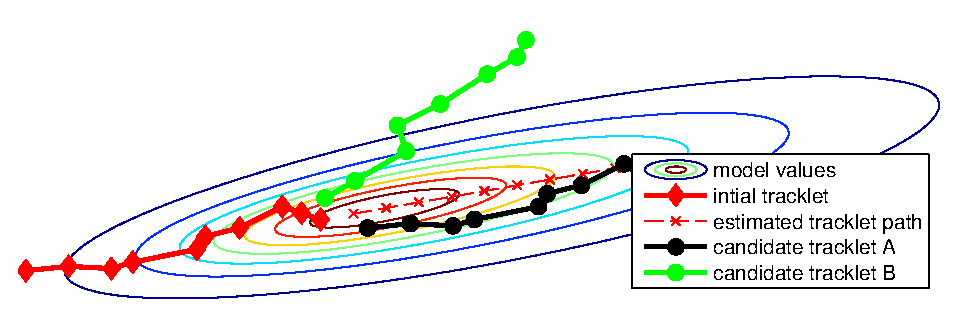
\includegraphics[width=\textwidth]{images/fig_gaussianbroadening1}
				\end{subfigure}%
				\hfill
				\begin{subfigure}{.2\textwidth}
				  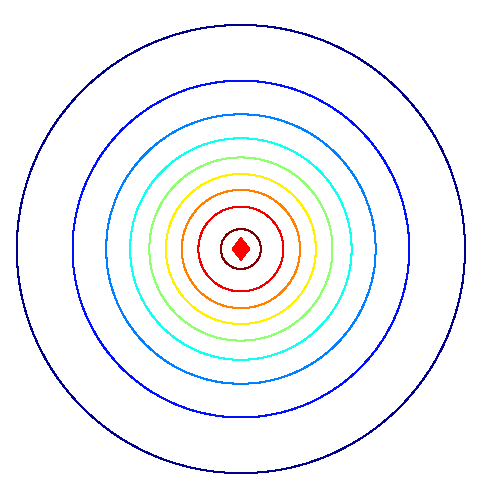
\includegraphics[width=\textwidth]{images/fig_gaussianbroadening2}
				\end{subfigure}
				\caption{Gaussian broadening feature. The distribution is computed for the red tracklet. The contour colours of the distribution are red for higher values and blue as the value decreases. The candidate black tracklet is given a linking likelihood of 0.20, while the green, which is angled from the direction of the red tracklet, a value of only 0.06. On the plot on the right we see that if a tracklet is composed of only one cell detection the value of the feature is equal all around it.}
				\label{fig:gaussianbroadening}
			\end{figure}
			
  		\subsection{Best feature selection \status{new}}
  			\label{sec:linkerbestfeatures}
	    	\notyetimplemented{}	    	
	    	\todo[inline]{Define how the best features have been selected}
	    	\todo[inline]{Describe which features performed best}